\documentclass[11pt,a4paper]{article}
\usepackage[english]{babel}
\renewcommand{\thesubsection}{\thesection.\alph{subsection}}

\usepackage{movie15}
\selectlanguage{english}
\NeedsTeXFormat{LaTeX2e}
\renewcommand{\baselinestretch}{1.3}
\usepackage[utf8]{inputenc}
\usepackage{enumerate}
\usepackage{listings}
\usepackage{amsmath}
\usepackage{amsfonts}
\usepackage{amssymb}
\usepackage{afterpage}
\usepackage{lscape}
\usepackage{caption}
\usepackage{appendix}
\usepackage{enumitem}
\usepackage{upquote}
\usepackage{xcolor}
\usepackage{graphicx}
\usepackage{fancyhdr}
\usepackage{makecell}
\usepackage{mdwlist}
%Mida de marges i columnes______
\usepackage{vmargin}
\usepackage{graphicx}
\graphicspath{ {imatges/} }
\setpapersize{A4}
\setmargins{2.5cm}{1.5cm}{16.5cm} {23.42cm}{32.54pt}{1cm}{0pt}{1.5cm} 
\usepackage{multicol}
\usepackage{multirow}
\usepackage{float}
\usepackage{cancel}
\usepackage{gensymb}
\setlength{\columnsep}{1cm}
%_______________________________
%Bibliografia
\bibliographystyle{apalike}
\renewcommand{\baselinestretch}{1.2}
\usepackage[urldate=long]{biblatex}
\bibliography{refs.bib}
\usepackage{url}
%_______________________________

%Capçalera_______________________
\pagestyle{fancy}
\fancyhead[L]{Navier-Stokes}
\fancyhead[R]{Aerodinàmica, Mecànica de Vol i Orbital
%\includegraphics[scale=0.2]{imatges/upc.png}}
}
\setlength{\headheight}{40pt} 
%________________________________

\usepackage[hidelinks]{hyperref}
\usepackage[all]{hypcap}

\newenvironment{imatge}
{\par\medskip\noindent\minipage{\linewidth}}
{\endminipage\par\medskip}

\lstset{language=Matlab,breaklines=true}


%Taules
\usepackage{tabularx}
\usepackage{longtable}
%\usepackage[table]{xcolor}
%\usepackage[table,xcdraw]{xcolor}
%\documentclass[xcolor=table]{beamer}
\usepackage{diagbox}

%Símbol €
\usepackage[utf8]{inputenc}
\usepackage{eurosym}


%Requadrar text
\usepackage{amsthm}
\usepackage{verbatim}

%Matlab
%\usepackage{listings}
\usepackage{matlab-prettifier}

%Annex
\usepackage{appendix}

%Totes les seccions del document_________________________
\begin{document}
\begin{titlepage}


\centering
{\bfseries\LARGE Universitat Politècnica de Catalunya\par}
%\vspace{1.5cm}
{\scshape\Large Escola Superior d'Enginyeries Industrial, Aeroespacial i Audiovisual de Terrassa\par}
\vspace{2.5cm}
{\scshape\Huge Assignment 1:  \\Numerical solution of the incompressible Navier-Stokes equations
 \par}
\vspace{2cm}
{\itshape\Large Aerodinàmica, Mecànica de Vol i Orbital \\ 2024-25 Q2 \par}
\vspace{0.5cm}
{06/04/2025 \par}
\vspace{0.5cm}
{\scshape\Large Group 12  \par}
\vspace{0.2cm}
{\Large Lluís Ceinos, Marc \par}
{\Large Gutiérrez Portillo, Guillem \par}
{\Large Poposki Stanojkovska, Vedran \par}
\vspace{2.5cm}
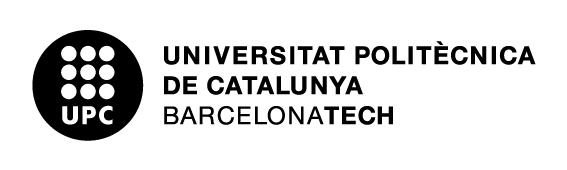
\includegraphics[width=0.4\textwidth]{imatges/logo upc negre sobre blanc.png}


\end{titlepage}
\newpage

% Índex___________________________
    %\addtocontents{toc}{\hfill \textbf{Page} \par}
    %\tableofcontents
    %\newpage
    %\listoffigures
    %\newpage
    %\listoftables
    %\newpage
%_________________________________
\section{Introduction to the Problem}

The objective of this problem is to determine the velocity and pressure fields as functions of spatial coordinates ($x, y$) and time ($t$) that satisfy the incompressible Navier-Stokes equations for arbitrary values of density ($\rho$) and kinematic viscosity ($\nu$). The problem is divided into the following parts:
\begin{itemize}
    \item \textbf{Part A:} Implementation and verification of the convective and diffusive terms. An analytic solution will be used and the goal is to show second order convergence.
    
    \item \textbf{Part B:} Implementation and verification of the pressure-velocity coupling. An arbitrary velocity field with non-null divergence is employed instead of $u^p$.
    
    \item \textbf{Part C:} Implementation and verification of time integration.
\end{itemize}

\subsection{Preliminary Considerations}
\begin{enumerate}
    \item \textbf{Staggered mesh:} The spatial discretization follows a staggered grid approach to avoid numerical instabilities and ensure proper representation of velocity and pressure fields.
    \item \textbf{Mesh for a periodic problem and halo update:} The domain is periodic, requiring careful treatment of boundary conditions and halo cells for data exchange between neighboring cells.
\end{enumerate}

\section{Part A}

This first part of the problem is intended to compute and verify the numerical computation of convective and diffusive terms using a known analytical solution. The goal is to demonstrate second-order convergence by computing numerical errors at different grid resolutions and checking their convergence.

\subsection{Algorithm}

Firstly, the intial condition is established a periodic velocity field as explained in the introduction. Then, the convective and diffusive terms for $u$ and $v$ are computed using symbolic differentiation.

The numerical computation is done for different grid resolutions ranging from 5 to 2560. The code loops over these grid sizes, repeating the following algorithm:

\begin{enumerate}
    \item Addition of halo and calculation of cell size.
    \item Computing numerical velocity field using set velocity field function with analytical $u$ and $v$ as inputs.
    \item Computing numerical convective and diffusive terms using the dedicated functions and the calculated velocity field.
    \item Compute analytical convective and diffusive fields on the grid
    \item Compute the maximum error for each computed field convective $u$, convective $v$, diffusive $u$ and diffusive $v$.
    \item Store errors in preallocated storage arrays.
    \item Plot errors.
\end{enumerate}

Custom functions have been developed to compute, among other things, the convective and diffusive terms. The calculation of the convective term is done by firstly interpolating the velocities at the faces, then computing flow terms and the convective terms for each velocity direction. In the case of the diffusive term, it is first approximated using second-order finite differences (forward and backward).

It is also important to highlight the importance of performing a halo update after each domain-wide computation. This means that at the halo update function is called at the end of each of the other implemented functions, updating the values of the cells at the edges of the domain.

\subsection{Validation strategy}

The basis for the validation of Part A is the comparison between numerical and analytical solutions for different grid sizes. The error between these two values is computed and plotted on a logarithmic scale, where it should appear with a slope of $h^2$ if it decreases quadratically, signifying second-order accuracy.

\subsection{Results}

\begin{figure}[H]
    \centering
    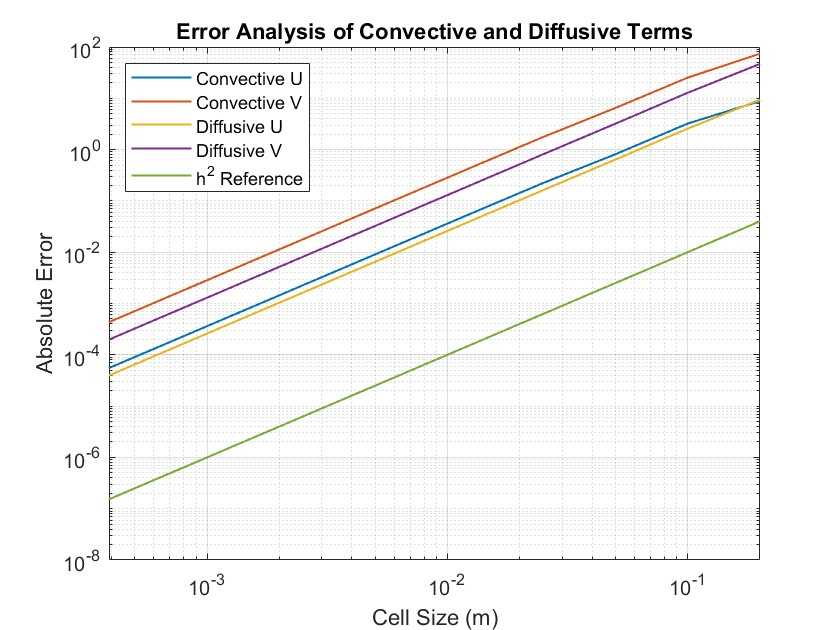
\includegraphics[width=0.7\linewidth]{imatges/PartAgraph.jpg}
    \caption{Error of computed terms}
    \label{fig:PartAError}
\end{figure}

The error lines are parallel to the $h^2$ reference, confirming second-order accuracy.
\section{Part B}

This second part of the problem aims to implement the pressure-velocity coupling and show how an arbitrary velocity field, after substracting the gradient of a certain type of field, can become a null-divergence one.

\subsection{Algorithm}

The implemented algorithm follows a simplified version of a predictor-corrector scheme. The objective is to begin with a velocity field containing artificial divergence and apply a correction using a scalar field (pseudo-pressure) whose gradient will subtract the divergence component from the velocity.

\begin{enumerate}
    \item Create coordinate positions, initialize null velocity field and introduce artificial divergence at a specific grid point by setting its horizontal and vertical velocities to non-zero values.
    \item Compute the divergence of the predictor velocity field using a custom function.
    \item Construct Laplacian matrix for pressure Poisson equation, solve a linear system for pseudo-pressure using the Laplacian equation and the divergence field in vector form.
    \item Convert the pseudo-P vector back to 2D field format, then compute its gradients. Correct the velocity field using the calculated pseudo-P gradients. Then, compute the divergence of this new velocity field.
    \item Compare maximum values of divergence before and after correction.
    \item Plot the results.
\end{enumerate}

A relevant remark about this code are that the divergence and gradient are calculated in the physical domain excluding the halo, which is calculated after. Both divergence and gradient are calculated using finite difference approximation, forward difference in the case of the gradient and backward for the divergence, ensuring consistency with the staggered-grid scheme.

\subsection{Validation strategy}

The validation of the pressure-velocity coupling is based on a two-step comparison of the divergence field. First, the divergence of the artificially perturbed velocity field is computed and its maximum absolute value is recorded. This provides a quantitative measure of how far the initial field is from being divergence-free. The maximum absolute divergence is again measured after correcting the velocity field.

A successful implementation should yield a corrected velocity field whose divergence is close to zero everywhere. Specifically, the maximum divergence should drop by several orders of magnitude, confirming that the projection step has effectively enforced incompressibility.

\subsection{Results}

\begin{figure}[H]
    \centering
    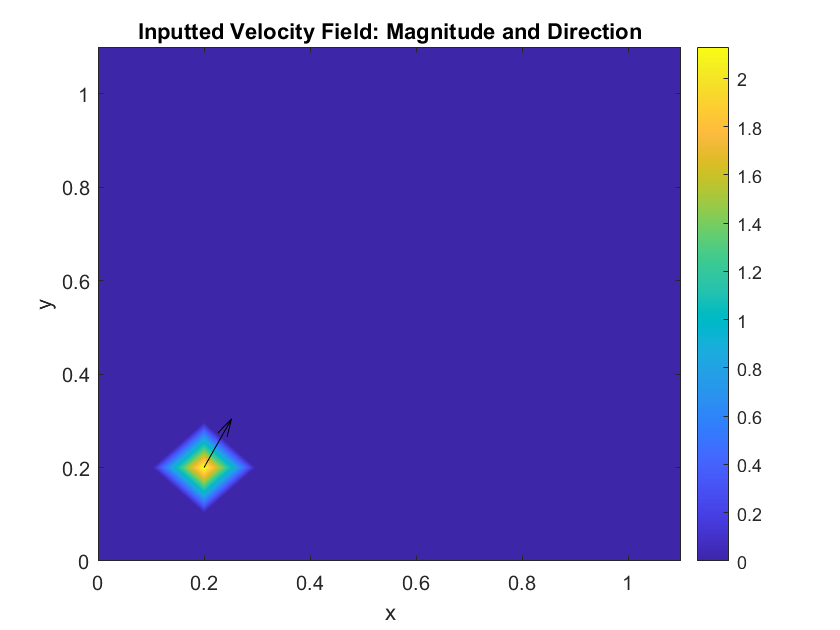
\includegraphics[width=0.7\linewidth]{imatges/InputV.png}
    \caption{Input non-zero velocity shown in the physical domain.}
    \label{fig:InputV}
\end{figure}

The visualization is consistent with with the injection of velocity in the null-velocity field.

\begin{figure}[H]
    \centering
    \includegraphics[width=0.7\linewidth]{imatges/PseudoP.png}
    \caption{Pseudo-pressure in the physical domain.}
    \label{fig:PseudoP}
\end{figure}

The pressure gradient is actively correcting the divergence introduced by the velocity. The gradient vectors align with regions of high pseudo-P variation.

\section{Part C}

\subsection{Algorithm and code}

\subsection{Validation strategy}

\subsection{Results}
\newpage

\section{\textbf{Conclusions}}

\bigskip

The study of non-viscous potential flows around different geometries, including a channel, a stationary cylinder, and a rotating cylinder, demonstrates the effectiveness of the numerical methodology in capturing fundamental flow characteristics. The comparison between analytical and numerical solutions for channel flow shows excellent agreement, confirming the accuracy of the numerical implementation for simple boundary conditions. In the case of flow around a stationary cylinder, the numerical results capture key features such as flow separation and stagnation points, though minor discrepancies are observed due to grid resolution limitations and numerical diffusion effects. The pressure distribution around the stationary cylinder aligns well with theoretical expectations, highlighting the symmetric nature of the potential flow and the absence of lift forces.

For the rotating cylinder case, the numerical solution successfully reproduces the overall circulation effects, with streamlines indicating the expected lift generation. However, discrepancies in the streamline pattern near the cylinder suggest that numerical diffusion and resolution of the vortex structure could be improved. The calculated lift and drag coefficients provide valuable insights into the aerodynamic forces acting on the cylinder, with results showing reasonable agreement with analytical predictions. 

Overall, the numerical methodology proves to be robust for modeling potential flow scenarios, providing useful approximations of analytical solutions. Further improvements, such as higher grid resolution, enhanced numerical schemes, and refined boundary condition handling, could lead to even better agreement with theoretical models, particularly for complex cases involving rotational effects.

\newpage
\printbibliography

%\appendix
%\newpage

\section{\textbf{Matlab Code}}



\bigskip

%Aquí el código


\end{document}
%________________________________________________________
